\documentclass[12px, a4paper]{article}
\usepackage[utf8]{inputenc}
% ~~~~~~~~~~~~~~~~~~~~~~~~~~~~~~~~~~~~~~~~~~~~~~~~~~~~~~~~~~~~~~~~~~~~~~~~~~~~~~
% Packages to be loaded before others
% ~~~~~~~~~~~~~~~~~~~~~~~~~~~~~~~~~~~~~~~~~~~~~~~~~~~~~~~~~~~~~~~~~~~~~~~~~~~~~~
%%% Packages for LaTeX - programming
%
% Define commands that don't eat spaces.
\usepackage{xspace}
% IfThenElse
\usepackage{ifthen}
%%% Doc: ftp://tug.ctan.org/pub/tex-archive/macros/latex/contrib/oberdiek/ifpdf.sty
% command for testing for pdf-creation
\usepackage{ifpdf} %\ifpdf \else \fi

%%% Internal Commands: ----------------------------------------------
\makeatletter
%
\providecommand{\IfPackageLoaded}[2]{\@ifpackageloaded{#1}{#2}{}}
\providecommand{\IfPackageNotLoaded}[2]{\@ifpackageloaded{#1}{}{#2}}
\providecommand{\IfElsePackageLoaded}[3]{\@ifpackageloaded{#1}{#2}{#3}}

\providecommand{\IfDefined}[2]{%
    \ifcsname #1\endcsname
    #2 %
    \else
    % do nothing
    \fi
}

\providecommand{\IfElseDefined}[3]{%
    \ifcsname #1\endcsname
    #2 %
    \else
    #3 %
    \fi
}
% Calculation with LaTeX
\usepackage{calc}
% Language setting
\usepackage[ngerman]{babel}
% Colors
\usepackage{xcolor}
% Graphics
\usepackage{graphicx}



% ~~~~~~~~~~~~~~~~~~~~~~~~~~~~~~~~~~~~~~~~~~~~~~~~~~~~~~~~~~~~~~~~~~~~~~~~~~~~~~
% Fonts
% ~~~~~~~~~~~~~~~~~~~~~~~~~~~~~~~~~~~~~~~~~~~~~~~~~~~~~~~~~~~~~~~~~~~~~~~~~~~~~~
\usepackage[T1]{fontenc}
% Additional Symbols (Text Companion font extension)
\usepackage{textcomp}



% ~~~~~~~~~~~~~~~~~~~~~~~~~~~~~~~~~~~~~~~~~~~~~~~~~~~~~~~~~~~~~~~~~~~~~~~~~~~~~~
% Math
% ~~~~~~~~~~~~~~~~~~~~~~~~~~~~~~~~~~~~~~~~~~~~~~~~~~~~~~~~~~~~~~~~~~~~~~~~~~~~~~
\usepackage{amsmath}



% ~~~~~~~~~~~~~~~~~~~~~~~~~~~~~~~~~~~~~~~~~~~~~~~~~~~~~~~~~~~~~~~~~~~~~~~~~~~~~~
% Symbols
% ~~~~~~~~~~~~~~~~~~~~~~~~~~~~~~~~~~~~~~~~~~~~~~~~~~~~~~~~~~~~~~~~~~~~~~~~~~~~~~
%%% for Math
%\usepackage{mathrsfs} %% Schreibschriftbuchstaben für den Mathematiksatz (nur Großbuchstaben)
%\usepackage{dsfont}   %% Double Stroke Fonts
%\usepackage[mathcal]{euscript} %% adds euler mathcal font
\usepackage{amssymb}
%\usepackage[Symbolsmallscale]{upgreek} % upright symbols from euler package [Euler] or Adobe Symbols [Symbol]
%\usepackage[upmu]{gensymb}             % Option upmu
%%% common
%\usepackage{wasysym}  %% Doc: http://www.ctan.org/tex-archive/macros/latex/contrib/wasysym/wasysym.pdf
%\usepackage{marvosym} %% Symbols from marvosym Font
%\usepackage{pifont}   %% ZapfDingbats



% ~~~~~~~~~~~~~~~~~~~~~~~~~~~~~~~~~~~~~~~~~~~~~~~~~~~~~~~~~~~~~~~~~~~~~~~~~~~~~~
% Text
% ~~~~~~~~~~~~~~~~~~~~~~~~~~~~~~~~~~~~~~~~~~~~~~~~~~~~~~~~~~~~~~~~~~~~~~~~~~~~~~
%%% Refs
\usepackage[ngerman]{varioref}
\usepackage{hyperref}
%%% Columns
\usepackage{multicol}



% ~~~~~~~~~~~~~~~~~~~~~~~~~~~~~~~~~~~~~~~~~~~~~~~~~~~~~~~~~~~~~~~~~~~~~~~~~~~~~~
% Graphics
% ~~~~~~~~~~~~~~~~~~~~~~~~~~~~~~~~~~~~~~~~~~~~~~~~~~~~~~~~~~~~~~~~~~~~~~~~~~~~~~
\usepackage[all]{xy}
\usepackage{float}
\usepackage{tikz}
%%% Doc: ftp://tug.ctan.org/pub/tex-archive/macros/latex/contrib/subfig/subfig.pdf
% Incompatible: loads package capt-of. Loading of 'capt-of' afterwards will fail therefor
\usepackage{subfig}



% ~~~~~~~~~~~~~~~~~~~~~~~~~~~~~~~~~~~~~~~~~~~~~~~~~~~~~~~~~~~~~~~~~~~~~~~~~~~~~~
% Captions & Style
% ~~~~~~~~~~~~~~~~~~~~~~~~~~~~~~~~~~~~~~~~~~~~~~~~~~~~~~~~~~~~~~~~~~~~~~~~~~~~~~
%%% Doc: ftp://tug.ctan.org/pub/tex-archive/macros/latex/contrib/caption/caption.pdf
\usepackage{caption}
% Aussehen der Captions fuer subfigures (subfig-Paket)
\IfPackageLoaded{subfig}{
    \captionsetup[subfloat]{%
        margin = 10pt,
        font = {small,rm},
        labelfont = {small,bf},
        format = plain, % oder 'hang'
        indention = 0em,  % Einruecken der Beschriftung
        labelsep = space, %period, space, quad, newline
        justification = RaggedRight, % justified, centering
        singlelinecheck = true, % false (true=bei einer Zeile immer zentrieren)
        position = bottom, %top
        labelformat = parens % simple, empty % Wie die Bezeichnung gesetzt wird
    }
}



% ~~~~~~~~~~~~~~~~~~~~~~~~~~~~~~~~~~~~~~~~~~~~~~~~~~~~~~~~~~~~~~~~~~~~~~~~~~~~~~
% Misc
% ~~~~~~~~~~~~~~~~~~~~~~~~~~~~~~~~~~~~~~~~~~~~~~~~~~~~~~~~~~~~~~~~~~~~~~~~~~~~~~
% Theorems
\usepackage{amsthm}
\newtheorem{Definition}{Definition}
\newtheorem{Beispiel}{Beispiel}
\newtheorem{Satz}{Satz}
\newtheorem{Bemerkung}{Bemerkung}
\newtheorem{Algorithmus}{Algorithmus}

% Listings
\usepackage{listings}
\definecolor{Brown}{cmyk}{0,0.81,1,0.60}
\definecolor{OliveGreen}{cmyk}{0.64,0,0.95,0.40}
\definecolor{CadetBlue}{cmyk}{0.62,0.57,0.23,0}
\definecolor{lightlightgray}{gray}{0.9}
\lstset{
    language=C,                             % Code langugage
    basicstyle=\rm\ttfamily,                % Code font, Examples: \footnotesize, \ttfamily
    keywordstyle=\color{OliveGreen},        % Keywords font ('*' = uppercase)
    commentstyle=\color{gray},              % Comments font
    numbers=left,                           % Line nums position
    numberstyle=\tiny,                      % Line-numbers fonts
    stepnumber=1,                           % Step between two line-numbers
    numbersep=5pt,                          % How far are line-numbers from code
    backgroundcolor=\color{lightlightgray}, % Choose background color
    frame=none,                             % A frame around the code
    tabsize=2,                              % Default tab size
    captionpos=b,                           % Caption-position = bottom
    breaklines=true,                        % Automatic line breaking?
    breakatwhitespace=false,                % Automatic breaks only at whitespace?
    showspaces=false,                       % Dont make spaces visible
    showtabs=false,                         % Dont make tabls visible
    %columns=flexible,                       % Column format
    %morekeywords={someword, otherword},     % specific keywords
}

\usepackage{amsmath}
\usepackage{hyperref}
\usepackage{float}

\begin{document}

%front
\title{ Angewandte Mathematik}
\author{Dr. Johannes Riesterer}
\date{\today}
\maketitle\thispagestyle{empty}
 \begin{figure}[H]
    \centering
    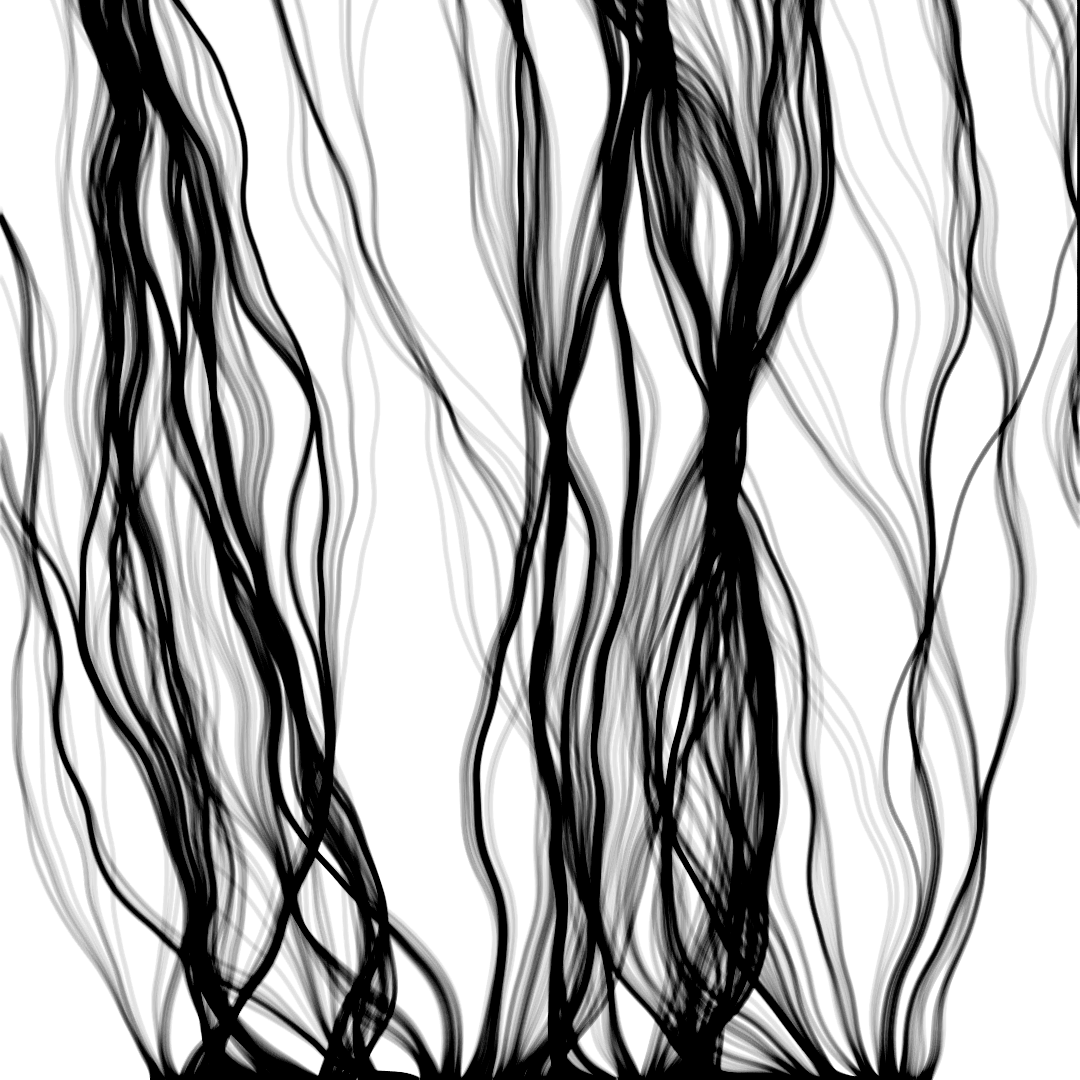
\includegraphics[width=1.0 \textwidth]{images/cover.png}
    \label{fig:diffus}
\end{figure}
\newpage 
\begin{center}
\large
 \copyright Johannes Riesterer \\
\end{center}
\thispagestyle{empty}
\newpage

\section*{Vorwort}
Kann jeder Mathematik lernen? Als Antwort auf diese Frage möchte ich auf den interessanten Lebenslauf
einer der bedeutendsten Mathematikerinnen aller Zeiten eingehen  (Auszug aus Wikipedia):

Emmy Noether war eine deutsche Mathematikerin, die grundlegende Beiträge zur abstrakten Algebra und zur theoretischen Physik lieferte. Insbesondere hat Noether die Theorie der Ringe, Körper und Algebren revolutioniert. Das nach ihr benannte Noether-Theorem gibt die Verbindung zwischen Symmetrien von physikalischen Naturgesetzen und Erhaltungsgrößen an. 

Sie zeigte in mathematischer Richtung keine besondere Frühreife, sondern hatte in ihrer Jugend Interesse an Musik und Tanzen. Sie besuchte die Städtische Höhere Töchterschule – das heutige Marie-Therese-Gymnasium – in der Schillerstraße in Erlangen. Mathematik wurde dort nicht intensiv gelehrt. Im April 1900 legte sie die Staatsprüfung zur Lehrerin der englischen und französischen Sprache an Mädchenschulen in Ansbach ab. 1903 holte sie in Nürnberg die externe Abiturprüfung am Königlichen Realgymnasium – dem heutigen Willstätter-Gymnasium – nach. 


\newpage

%Einfügen des Inhaltsverzeichnisses
\tableofcontents
\newpage
\thispagestyle{empty}
\mbox{}\thispagestyle{empty}
\newpage
%main

\section{Vorwissen und Konventionen}

\subsubsection*{Differenzierbarkeit reeller Funktionen} 
Eine reelle Funktion $f : (a, b) \to \mathbb{R}$  heißt differenzierbar in $x \in (a,b)$, falls der Grenzwert $\lim_{h \to 0}  \frac{f(x +h) - f(x)}  {h}$ existiert. In diesem Fall heißt dieser Grenzwert die Ableitung (Steigung) von $f$ in $x$ und wird mit $f' (x)$ bezeichnet.
\begin{figure}[H]
      \centering
    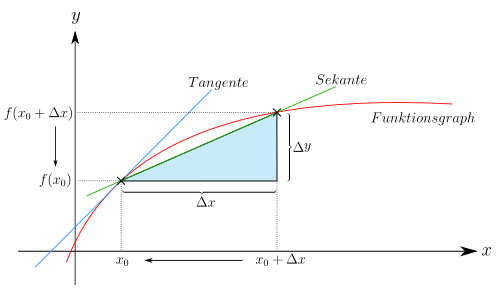
\includegraphics[width=0.8\textwidth]{images/Differencial_quotient_of_a_function}
      \caption{Quelle: Wikipedia: https://de.wikipedia.org/wiki/Datei:Differencial\_quotient\_of\_a\_function.svg}
\end{figure}

\subsubsection*{Mittelwertsatz einer Veränderlichen} 

Sei $f : [a,b] \to \mathbb{R}$ stetig und differenzierbar für alle $x \in (a,b)$. Dann gibt es $\xi \in (a,b)$ mit
$f'(\xi) = \frac{f(b) - f(a)} { b-a}$.
\begin{figure}[H]
      \centering
    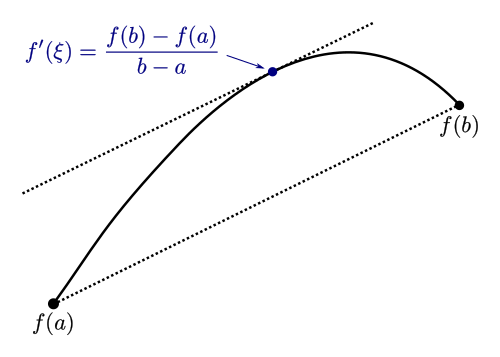
\includegraphics[width=0.6\textwidth]{images/Mittelwertsatz3.png}
      \caption{Quelle: Wikipedia: https://commons.wikimedia.org/wiki/File:Mittelwertsatz3.svg}
\end{figure}

\subsubsection*{Taylorapproximation einer Veränderlichen} 

Jede  reelle Funktion $f$, deren $p+1$-ten Ableitungen existieren und stetig sind lässt sich mit Hilfe der Taylorreihe  $$f(x) = f(a) + \frac{1}{2!} f^{'} (x-a) +   \frac{1}{3!} f^{''}(a) (x-a)^2 + \cdots  +  \frac{1}{p!} f^{(p)}(a) (x-a)^{p-1} +  R_{p+1}(x,a) $$
und dem Restglied  $R_p(x,a) :=   \frac{1}{(p+1)!} f^{(p+1)}(\xi) (x-a)^{p} $ mit einem $\xi \in (x,a)$ darstellen.


\subsubsection*{Cauchy-Schwarzsche Ungleichung}
 Für zwei Vektoren $v,w \in \mathbb{R}^n$ gilt: 
\begin{align*}
\frac{\langle v, w \rangle}{||v|| \cdot ||w||} = \cos(\varphi) 
\end{align*}
wobei $\varphi$ der Innenwinkel zwischen $v$ und $w$ ist.

\subsubsection*{Äquivalenz von Normen}
 Die Normen $||v||: = \sqrt{\sum_{i = 1}^n v_i^2}$ und $||v||_{\infty}:= \max \{ v_1, \cdots, v_n \} $ sind Äquivalent. Sie lassen sich  mit Konstanten $k_1 ||v|| < ||v||_{\infty} k_2  ||v|| $ gegeneinander abschätzen.

\subsubsection*{Symmetrische Matrizen}
 Für eine symmetrische Matrix $A \in \mathbb{R}^{n \times n}$ ist Äquivalent:
\begin{itemize}
\item $A$ hat positive Eigenwerte.
\item $v^TA v > 0$ für alle $v \neq 0$.
\item alle Unterdeterminanten sind positiv. Speziell für $n=2$ und $A = \begin{pmatrix} a & b \\ b & d\end{pmatrix}$ bedeutet dies
$a >0$ und $ad -b^2 >0$. 
\end{itemize}

\begin{Definition}[Konventionen]
In diesem Abschnitt ist $U \subset \mathbb{R}^n$ stets eine offene Teilmenge des $\mathbb{R}^n$.
 $e_i := \begin{pmatrix}  0 \\  \vdots \\ 1  (\text{i-te Zeile})\\ \vdots \\ 0 \end{pmatrix}$  bezeichnet den $i$-ten Basisvektor des $\mathbb{R}^n$.

\end{Definition}

\section{Mehrdimensionale Differentialrechnung}

\begin{Definition}[Konvergenz]
 Eine Folge $(a_n)$ in $\mathbb{R}^n$ heißt konvergent gegen den Grenzwert $a \in \mathbb{R}^n$, wenn gilt:
\begin{align*}
\forall {\varepsilon > 0} \ \exists \ N \in \mathbb{N} \; \forall \ n > N: \; d(a, a_n) < \varepsilon\,
\end{align*}
In Worten: Es gibt für jedes beliebige (noch so kleine) $\varepsilon$ einen Index $N$ derart, dass für alle Indizes $n > N$, also alle weiteren Folgenglieder, gilt: Der Abstand $d(a, a_n)$ ist kleiner als $\varepsilon$.
\end{Definition}

\begin{figure}[H]
      \centering
    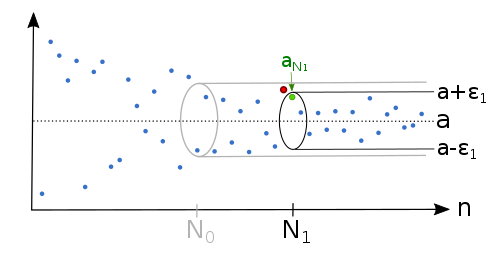
\includegraphics[width=0.9\textwidth]{images/500px-Epsilonschlauch_klein}
      \caption{Quelle: Wikipedia: https://commons.wikimedia.org/wiki/File:Epsilonschlauch\_klein.svg}
\end{figure}



\begin{Definition}[Grenzwert]
Sei $f :X \subset \mathbb{R}^n \to \mathbb{R}^m$ eine  Funktion und $a \in X$. Wir nennen $L_a \in \mathbb{R}^m$ Grenzwert von $f$ bezüglich der Annäherung von $x$ an $a$, falls für jede  konvergente Folge $x_n \to a$  die Folge $f(x_n)$ nach $L_a$ konvergiert.  In diesem Fall bezeichnen wir
\begin{align*}
\lim_{x \to a} f(x) = L_a \;.
\end{align*}
Dies ist gleichbedeutend damit, dass für jedes $\epsilon > 0$ ein $\delta > 0$ existiert, so dass
$d(f(x) ,L_a) < \epsilon$ gilt für jedes $x$ mit $d(x, a) < \delta$.
\end{Definition}


\begin{figure}[H]
      \centering
    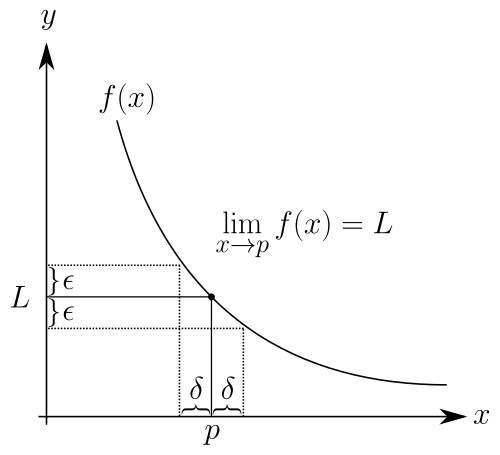
\includegraphics[width=0.6\textwidth]{images/500px-Limes_Definition_Vektorgrafik}
      \caption{Quelle: Wikipedia: https://de.wikipedia.org/wiki/Datei:Limes\_Definition\_Vektorgrafik.svg}
    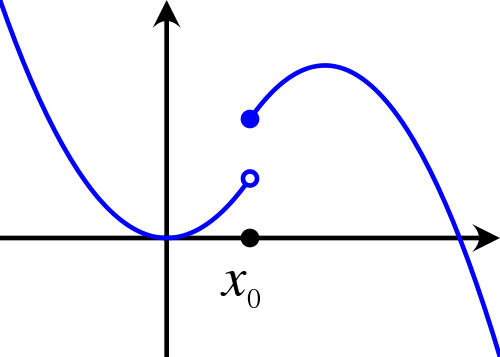
\includegraphics[width=0.6\textwidth]{images/500px-Upper_semi}
      \caption{Quelle: Wikipedia: https://commons.wikimedia.org/wiki/File:Upper\_semi.svg}
\end{figure}




\begin{Definition}[Stetige Funktion]
Eine reellwertige Funktion $f :U \to \mathbb{R}$ heißt stetig, wenn für alle $y \in U$ der Grenzwert $\lim_{x \to y} f(x) = L_{y} $ existiert.
\end{Definition}


\subsection{Richtungsableitung und Gradient reellwertiger Funktionen}
Ableitungen beschreiben bildlich gesprochen das Verhalten einer Funktion bezüglich beliebig kleiner Änderungen der Eingabewerte.





\begin{Definition}[Richtungsableitung]
Sei $f: U \to \mathbb{R}$ eine Funktion. Für einen Vektor $h \in  \mathbb{R}^n$, $t \in \mathbb{R}$  und einen Punkt  $a \in U$ heißt der Grenzwert (falls er existiert) 
\begin{align*}
\partial_h f(a) := \lim_{t \to 0} \frac{f(a + th) - f(a)}{t}
\end{align*}
Richtungsableitung von $f$ am Punkt $a$ in Richtung $h$. Sie misst die Änderung der Funktion in Richtung $h$.

Speziell nennen wir für die Standard Basisvektoren $e_i$ 
\begin{align*}
\frac{\partial f(a)}{\partial x_i}  := \partial_{e_i} f(a) := \lim_{t \to 0} \frac{f(a + t e_i) - f(a)}{t}
\end{align*}
die partielle Ableitung von $f$ in $a$ nach $x_i$.
\end{Definition}

\begin{Definition}[Partielle Differenzierbarkeit]
Eine Funktion  $f: U \to \mathbb{R}$ heißt partiell differenzierbar im Punkt $a \in U$, falls alle partiellen Ableitungen 
$$\frac{\partial f(a)}{\partial x_1}, \cdots , \frac{\partial f(a)}{\partial x_n}$$ 
existieren.
\end{Definition}

\begin{Definition}[Differenzierbarkeit]
\label{diffbarkeit}
Eine Funktion $f: U \to \mathbb{R}$ heißt  differenzierbar im Punkt $a \in U$, falls alle partiellen Ableitungen 
$$\frac{\partial f(a)}{\partial x_1}, \cdots, \frac{\partial f(a)}{\partial x_n}$$
 existieren und stetig sind.  Mann nennt  in diesem Fall die $1 \times n$-Matrix 
$$df(a) := \biggl( \frac{\partial f(a)}{\partial x_1}, \cdots, \frac{\partial f(a)}{\partial x_n} \biggr)$$
das Differential von $f$ im Punkt $a$. Der Vektor 
$$\nabla f (a) := \begin{pmatrix}  \frac{\partial f(a)}{\partial x_1} \\  \vdots \\ \frac{\partial f(a)}{\partial x_n}  \end{pmatrix}$$
wird als Gradient bezeichnet. Es ist $df(a) \cdot h = \langle \nabla f (a) , h \rangle$.
\end{Definition}

\fbox{\parbox{\linewidth}{
$\star \star \bigstar $  Der Unterschied zwischen  Differenzierbarkeit und partieller Differenzierbarkeit ist also, dass die partiellen Ableitungen zusätzlich  zur Existenz auch stetig sein müssen.
}}

\begin{figure}[H]
      \centering
    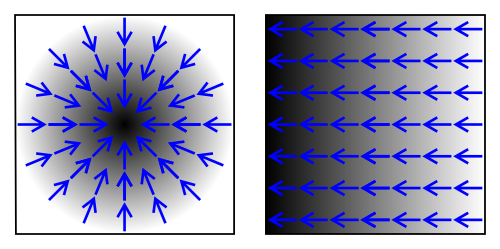
\includegraphics[width=1.0\textwidth]{images/Gradient}
      \caption{Quelle: Wikipedia: https://commons.wikimedia.org/wiki/File:Gradient2.svg}
\end{figure}


\begin{Bemerkung}
\label{partial1}
Für das Differential einer differenzierbaren Funktion  $f: U \to \mathbb{R}$ gilt für alle $a \in U$:
\begin{itemize}
\item  $df(a) (h) :=  df(a) \cdot h$ ist eine lineare Abbildung von $\mathbb{R}^n$ nach $\mathbb{R}$.
\item $df(a)  \cdot h = \partial_h f(a)$. 
\item $d (f \cdot g) = g(a) d(f) + f(a) dg$
\item $d(f + g) = df + dg$
\end{itemize}
\end{Bemerkung}
\begin{proof}
\begin{itemize}
\item  Multiplikation mit einer Matrix ist eine lineare Abbildung.
\item Für die Basisvektoren ist per Definition $df(a)  \cdot e_i = \partial_{e_i} f(a)$. Da jeder Vektor $h$ eine Linearkombination der Basisvektoren ist und $df$ linear ist, folgt die Behauptung.
\item Folgt direkt aus der entsprechenden Eigenschaft reeller Funktionen.
\item Folgt direkt aus der entsprechenden Eigenschaft reeller Funktionen.
\end{itemize}
\end{proof}


\begin{Satz}[Steilste Anstiegsrichtung]
Sei   $f: U \to \mathbb{R}$ differenzierbare Funktion,  $a \in U$ und $v := \text{argmax}_{ h \in S^n} \partial_h f(a) $.
Dann gilt 
\begin{align*}
|| \nabla f(a) || v =  \nabla f(a) \; .
\end{align*} 
\end{Satz}
\begin{proof}
Mit der CSU Ungleichung folgt für beliebiges $h$ 
\begin{align*}
\partial_h f(a) = df(a) h = \langle \nabla f(a) , h \rangle = || \nabla f(a)||  \cdot ||h|| \cdot \cos(\varphi) 
\end{align*} 
wobei $\varphi$ den Innenwinkel zwischen $\nabla f(a)$ und $h$ bezeichnet. Für $||h|| = 1$ wird somit $\partial_h f(a) $ maximal, wenn $\varphi = 0$ und somit $h =  \frac{\nabla f(a)}{||\nabla f(a)||}$ ist.
\end{proof}





%-----------------------------------------------------
% Ende VL 1
%-----------------------------------------------------


\begin{Satz}[Lokale Linearisierung]
\label{lokaleLinearisierung}
Ist  $f: U \to \mathbb{R}$ differenzierbar, so gibt es ein Restglied $R(h)$ mit  $\lim_{h \to 0} \frac{R(h)}{ ||h||} = 0$  so dass für alle $a \in U$ und $h \in \mathbb{R}$ 
\begin{align*}
f(a + h)  =  f(a)  +  df(a) \cdot h + R(h) 
\end{align*}
gilt. 
\end{Satz}

\fbox{\parbox{\linewidth}{
$\star \star \bigstar $ Eine differenzierbare Funktion kann  auf hinreichend kleinen Umgebungen  \\
beliebig genau durch eine lineare Funktion approximiert werden. 
}}

\fbox{\parbox{\linewidth}{
$\diamond \Diamond $  Der Beweis beruht im Wesentlichen auf dem Mittelwertsatz einer Veränderlichen.
}}


\begin{proof}
Wir wählen einen offenen, achsenparallelen Quader $Q \subset U$, so dass er vollständig in $U$ enthalten und $a \in Q$ ist.
Jeder Punkt $a + h \in Q$  lässt sich damit durch einen achsenparallelen Streckenzug durch die Punkte
\begin{align*}
& a_0 := a \\
& a_i  := a_{i-1} + h_i e_i;  \;  \;  i = 1, \cdots , n
\end{align*} 
mit $a$ verbinden. 
\begin{figure}[H]
      \centering
    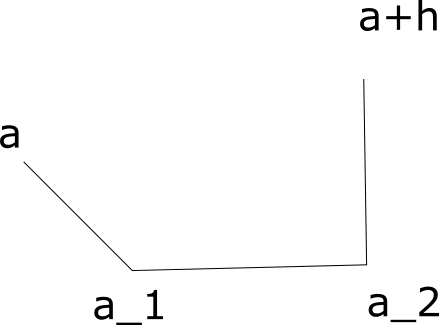
\includegraphics[width=0.4\textwidth]{images/kantenzug}
      \caption{Kantenzug mit achsenparallelen Kanten}
\end{figure}

Damit ist $f(a + h) - f(a) = \sum_{i=1}^{n} \bigl( f (a_i)   - f(a_{i-1})   \bigr)$ und  mit $\varphi_i(t) : = f(a_i + t e_i)$ gilt 
$f(a_i) - f(a_{i-1}) = \varphi_i(h_i)  - \varphi_i(0)$. Wegen dem Mittelwertsatz einer Veränderlichen gibt  es  $\tau_i$  mit
\begin{align*}
\varphi_i(h_i)  - \varphi_i(0)  = h_i \varphi'(\tau_i) \;.
\end{align*} 
Da $\varphi'_i(t) = \frac{\partial  f(a_{i-1} + t e_i ) }{\partial x_i}$ folgt mit $\xi_i: = a_i + \tau_i e_i$ 

\begin{align*}
f(a + h) - f(a) - df(a) \cdot h = \sum_{i=1}^n  \biggl( \frac{\partial  f(\xi) }{\partial x_i} -    \frac{\partial  f(a) }{\partial x_i}   \biggr) h_i
\end{align*} 
und damit
\begin{align*}
| f(a + h) - f(a) - df(a) \cdot h |  \leq || h ||_{\infty}  \sum_{i=1}^n  \biggl| \frac{\partial  f(\xi) }{\partial x_i} -    \frac{\partial  f(a) }{\partial x_i}   \biggr | \; . 
\end{align*} 
Für $h \to 0$ gilt $\xi_i \to a$ und da die partiellen Ableitung stetig sind nach Voraussetzung und alle Normen äquivalent sind folgt

\begin{align*}
\lim_{h \to 0} \frac{ f(a + h) - f(a) - df(a) \cdot h}{||h||} = 0 
\end{align*} 
und damit die Behauptung.
\end{proof}

\begin{Bemerkung}
\label{differentialeindeutig}
Umformuliert bedeutet Satz \ref{lokaleLinearisierung}, dass für das Differential einer differenzierbare Funktion
\begin{align}
\lim_{h \to 0} \frac{f(a + h) -f(a) - df(a) h }{||h||} = 0
\end{align}
Ist $L$ eine weiter lineare Abbildung mit $\lim_{h \to 0} \frac{f(a + h) -f(a) - L(a) h }{||h||}$, so ist $L = df$. Das Differential ist somit eindeutig durch die Eigenschaft der lokalen Linearisierung bestimmt.
\end{Bemerkung}
\begin{proof}
Für $v \in \mathbb{R}^n$ mit $||v|| = 1$ gilt 
\begin {align*}
\bigl( L(a) - df(a) \bigr)(v) =  \lim_{t \to 0}  \bigl( L(a) - df(a) \bigr) \bigl( \frac{tv}{||tv||} \bigr) = \lim_{t \to 0} \frac{\bigl( L(a) - df(a) \bigr)(tv) }{||tv||} = 0
\end{align*}
\end{proof}

\begin{Definition}[Differenzierbarer Weg]
Seien $a,b \in \mathbb{R}$. Ein Weg ist eine Abbildung  
\begin{align*}
& \gamma:  [a,b] \to \mathbb{R}^n \\
& \gamma (t) :=  \begin{pmatrix} \gamma_1(t) \\ \vdots \\ \gamma_n(t) \end{pmatrix}
\end{align*}
mit reellen, stetigen Funktionen $y_i : [a,b] \to \mathbb{R}$ (damit ist auch $\gamma$ stetig). Der Weg heißt differenzierbar, falls alle Ableitungen $\gamma_i'(t)$ existieren. In diesem Fall definieren wir
\begin{align*}
 \gamma' (t) :=  \begin{pmatrix} \gamma'_1(t) \\ \vdots \\ \gamma'_n(t) \end{pmatrix}
\end{align*}
\end{Definition}

\begin{figure}[H]
      \centering
    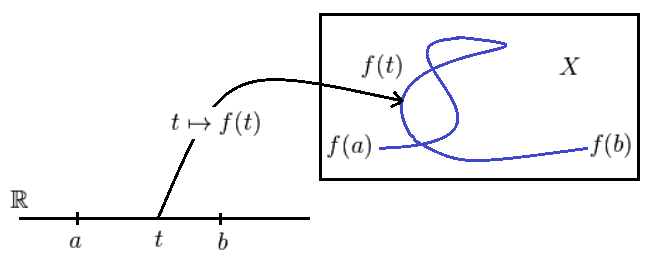
\includegraphics[width=0.8\textwidth]{images/EbeneKurve}
      \caption{Quelle: Wikipedia: https://de.wikipedia.org/wiki/Datei:EbeneKurve.png}
\end{figure}
Im Folgenden gilt: $I := [a, b]$ mit $a,b \in \mathbb{R}$ und $U \subset \mathbb{R}^n$.
\begin{Satz}[(Baby) Kettenregel]
Sei $\gamma: I \to U$ ein differenzierterer Weg und $f: U \to \mathbb{R}$ eine differenziertere Funktion. Dann ist $f \circ \gamma : I \to \mathbb{R}$ differenzierbar und hat die Ableitung
\begin{align*}
\frac{d(f \circ \gamma)}{dt}(t) = df(\gamma(t))\gamma'(t) = \sum_{i=1}^n  \frac{\partial f (\gamma(t))}{\partial x_i} \gamma'_i(t)
\end{align*} 
\end{Satz}

\fbox{\parbox{\linewidth}{
$\star \star \bigstar $  Das Differential einer differenzierteren Funktion  kann als eine Abbildung von Tangenten interpretiert werden.
}}

\begin{proof}
Wegen der Differenzierbarkeit des Weges und der Funktion gilt für hinreichend kleine $k \in \mathbb{R}$ und $h \in \mathbb{R}^n$
\begin{align*}
& \gamma (t + k) = \gamma(t) + k \gamma'(t) + r_1 (k) |k|, \text{ mit } lim_{k \to 0} r_1(k) = 0  \\
& f(\gamma(t) + h) = f(\gamma(t)) + df(\gamma(t)) \cdot \gamma'(t) h +  r_2 (h)  ||h|| , \text{ mit } lim_{h \to 0} r_2(h) = 0 
\end{align*} 
 Mit $h:= \gamma(t + k) - \gamma(t)$ folgt
\begin{align*}
f(\gamma(t + k)) = f(\gamma(t)) + df(\gamma(t)) \cdot \gamma'(t) k +  R(k)
\end{align*}  
mit dem Restglied
\begin{align*}
R(k) := df(\gamma(t)) r_1(k) |k| + r_2 \bigl( \gamma (t + k) - \gamma(t) \bigr) ||\gamma'(t) k + r_1(k) |k| || 
\end{align*}  
Da $\lim_{k \to 0} R(k) = 0$ folgt die Behauptung.
\end{proof}




\begin{Satz}[Mittelwertsatz]
Sei $f :U \to \mathbb{R}$ eine differenziertere Funktion und $a, b \in U$, so dass die Verbindungsstrecke von $a$ nach $b$ vollständig in $U$ liegt. 
Dann gibts es einen Punkt $\xi \in [a,b]$ mit
$$f(b) - f(a) = df(\xi) (b-a) \; .$$ 
\end{Satz}
\begin{figure}[H]
      \centering
    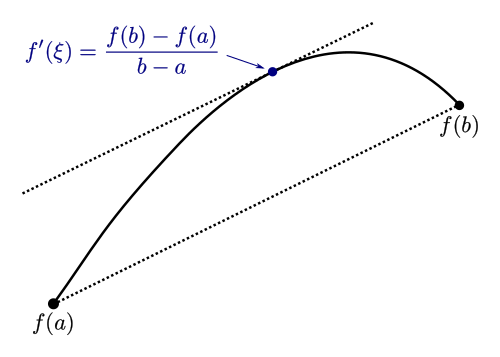
\includegraphics[width=0.6\textwidth]{images/Mittelwertsatz3.png}
      \caption{Quelle: Wikipedia}
\end{figure}
\begin{proof}
Setze $\gamma(t) := a + t(b-a), \; t \in [0,1]$ (Verbindungsgerade zwischen $a$ und $b$) und $F : = f  \circ \gamma : [0,1] \to \mathbb{R}$.
Damit ist $F(1)- F(0) = f(1) - f(0)$ und nach der Kettenregel ist $F$ differenzierbar.  Mit dem Mittelwertsatz einer Veränderlichen gibt es $\tau \in (0,1)$ mit 
$F(1) - F(0) = F'(\tau) = df(\gamma (\tau)) (b-a)$. Somit ist $\xi := \gamma(\tau)$ der gesuchte Punkt.
\end{proof}


\begin{Satz}[Satz von Schwarz]
Wenn Für eine Funktion $f: U \to \mathbb{R}$ die Ableitungen $\frac{\partial}{\partial x_i} f(a)$, $\frac{\partial}{\partial x_j}f(a)$ und $ \frac{\partial}{\partial x_i}\frac{\partial }{\partial x_j} f(a)$ existieren und letztere stetig ist, dann existiert auch $ \frac{\partial}{\partial x_j}\frac{\partial }{\partial x_i} f(a)$ und es gilt
\begin{align*}
\frac{\partial}{\partial x_i}\frac{\partial }{\partial x_j} f(a) = \frac{\partial}{\partial x_j}\frac{\partial }{\partial x_i} f(a)
\end{align*}
\end{Satz}

\fbox{\parbox{\linewidth}{
$\star \star \bigstar $  Bei wiederholten Ableiten spielt die Reihenfolge keine Rolle, wenn eine der Ableitungen existiert und stetig ist.
}}

\fbox{\parbox{\linewidth}{
$\diamond \Diamond $  Der Beweis geht in zwei Schritten: Man wendet den Mittelwertsatz einer Veränderlichen auf eine Hilfsfunktion an. Damit kann man die Differenz der Ableitungen abschätzen und zeigen, dass sie beliebig klein wird und damit gleich sind.
}}

\begin{proof}
Setze $\varphi(x,y) := f(a + x e_i + y e_j)$ mit $(x,y) \in  V \subset \mathbb{R}^2$. Bei hinreichend kleiner Wahl von $V$ existieren die Ableitungen $ \frac{\partial}{\partial y} \varphi$, $ \frac{\partial}{\partial x} \varphi$ und $ \frac{\partial}{\partial y} \frac{\partial}{\partial x} \varphi$  existiert und ist stetig nach Voraussetzung an $f$. Es reicht nun zu zeigen, dass $ \frac{\partial}{\partial x} \frac{\partial}{\partial y} \varphi (0,0)$ existiert  und 
\begin{align*}
\frac{\partial}{\partial x} \frac{\partial}{\partial y} \varphi(0,0) = \frac{\partial}{\partial y} \frac{\partial}{\partial x} \varphi (0,0)
\end{align*} 
gilt.  Sei dazu $\epsilon > 0$ und $V' \subset V$ so gewählt, dass $| \frac{\partial}{\partial y} \frac{\partial}{\partial x} \varphi(x,y) -  \frac{\partial}{\partial y} \frac{\partial}{\partial x} \varphi(0,0) | < \epsilon$ gilt für $(x,y) \in V'$.
Innerhalb eines achsenparallelen Quaders $Q \subset V'$  mit Ecken $(0,0)$ und $(h,k)$ setzen wir $u(x) := \varphi(x,  k) - \varphi(x, 0)$. Zweimaliges Anwenden des Mittelwertsatzes einer Veränderlichen liefert  
\begin{align*}
& u(h) - u(0) = hu'(\xi) \\
& = h(  \frac{\partial}{\partial x} \varphi(\xi, k) - \frac{\partial}{\partial x} \varphi(\xi, 0) ) = h k \frac{\partial}{\partial y} \frac{\partial}{\partial x} \varphi(\xi, \eta) \; .
\end{align*}
Damit erhalten wir die Abschätzung 
\begin{align*}
\biggl | \frac{ u(h) - u(0)}{hk} -   \frac{\partial}{\partial y} \frac{\partial}{\partial x} \varphi (0,0) \biggr | < \epsilon \; .
\end{align*}
Da 
\begin{align*}
& \lim_{k \to 0 } \frac{ u(h) - u(0)}{hk} =  \lim_{k \to 0 } \frac{1}{h} \biggl(   \frac{\varphi(h,k) - \varphi(h,0)  }{k}  -\frac{\varphi(0,k) - \varphi(0,0)  }{k} \biggr) \\
& =   \biggl(   \frac{  \frac{\partial}{\partial y} \varphi(h,0) -   \frac{\partial}{\partial y}\varphi(0,0)  }{k} \biggr) 
\end{align*}
und 
\begin{align*}
& \lim_{h \to 0 } \biggl(   \frac{  \frac{\partial}{\partial y} \varphi(h,0) -   \frac{\partial}{\partial y}\varphi(0,0)  }{k} \biggr) 
 =     \frac{\partial}{\partial x} \frac{\partial}{\partial y} \varphi(0,0) 
\end{align*}
folgt die Behauptung.
\end{proof}

\subsubsection*{Anwendung: Taylorreihe} 


\begin{Definition}[ $\mathcal{C}^k$-Funktion]
Eine  Funktion  $f: U \to \mathbb{R}$ für die alle partiellen Ableitungen 
\begin{align*}
 \frac{\partial}{\partial x_{i_1}} \cdots   \frac{\partial}{\partial x_{i_k}} f(a)
\end{align*}
mit $i_1 + \cdots + i_k \leq k$ existieren und stetig sind heißt $\mathcal{C}^k$-Funktion oder $k$-mal stetig differenzierbar. Eine 
$\mathcal{C}^1$-Funktion ist also eine differenzierbare Funktion.
\end{Definition}

\begin{Definition}[Höhere Ableitungen]
Für  eine Funktion  $f: U \to \mathbb{R}$, $a \in U$ und Vektoren $v^1, \cdots , v^p \in \mathbb{R}^n$ heißt 
\begin{align*}
d^pf(a) \bigl(v^1, \cdots , v^p  ) := \partial_{v^1} \hdots \partial_{v^p} f(a)
\end{align*}
die $p$-te Richtungsableitung von $f$. Sie ist wegen dem Satz von Schwarz wohldefiniert.
Mit Bemerkung \ref{partial1} ist
\begin{align*}
d^pf(a) \bigl(v^1, \cdots , v^p  ) = \sum_{i_1 = 1}^n \cdots \sum_{i_p = 1}^n  \frac{\partial}{\partial x_{i_1}} \hdots \frac{\partial}{\partial x_{i_p}} f(a) \cdot v^1_{i_1} \cdots v^p_{i_p} \; .
\end{align*}
Für einen Vektor $z \in \mathbb{R}^n$ definieren wir $$d^pf(a) z^p := d^pf(a) \underbrace{(z, \cdots , z)}_{p-mal} \;.$$

\end{Definition}



\begin{Bemerkung}
Für $p = 2$ und $u,v \in \mathbb{R}^n$ ist
\begin{align*}
d^2f(a) \bigl(u , v ) = \sum_{i = 1}^n \sum_{j = 1}^n \frac{\partial}{\partial x_{i}}  \frac{\partial}{\partial x_{j}} f(a) v_{i}  u_{j} 
\end{align*}
und mit 
\begin{align*}
f''(a) : = \begin{pmatrix}  \frac{\partial}{\partial x_{1}} \frac{\partial}{\partial x_{1}} f(a)   &  \cdots &  \frac{\partial}{\partial x_{1}} \frac{\partial}{\partial x_{n}} f(a) \\
\vdots & & \vdots  \\
 \frac{\partial}{\partial x_{n}} \frac{\partial}{\partial x_{1}} f(a)   &  \cdots &  \frac{\partial}{\partial x_{n}} \frac{\partial}{\partial x_{n}} f(a)
\end{pmatrix} 
\end{align*}
ist $d^2f(a) \bigl(u , v ) = u^T  \cdot f''(a) \cdot v$. Die Matrix $f''(a)$ wird auch Hesse-Matrix genannt. Nach dem Satz von Schwarz ist sie symmetrisch.
\end{Bemerkung}


\begin{Satz}[Taylorapproximation]
Sei   $f: U \to \mathbb{R}$ eine $\mathcal{C}^{p+1}$-Funktion und $x,a \in U$, so dass die Verbindung zwischen $x$ und $a$ in $U$ liegt.
Dann gilt
\begin{align*}
f(x) = f(a) + \sum_{k=1}^{p} d^k f(a) (x-a)^k + R_{p+1} (x;a)
\end{align*}
mit dem Restglied $R_{p+1} (x;a) := \frac{1}{(p+1)!} d^{p+1}f(\xi) (x-a)^{p+1}$ für ein $\xi \in [a,x]$.
\end{Satz}

\begin{proof}
Sei $h := (x-a)$ und $F(t) := f(a + th)$ mit $t \in [0,1]$. Wiederholte Anwendung der (Baby) Kettenregel mit $\gamma(t) := a +th$ ergibt
\begin{align*}
& F'(t) = \sum_{i=1}^n  \frac{\partial}{\partial x_{i}} f(a + th) h_i \\
& F''(t) =\sum_{j=1}^n \sum_{i=1}^n   \frac{\partial}{\partial x_{j}} \frac{\partial}{\partial x_{i}} f(a + th) h_i h_j \\
& \vdots \\
& F^p(t) =  \sum_{i_1=1}^n  \cdots \sum_{i_p=1}^n   \frac{\partial}{\partial x_{i_1}} \cdots \frac{\partial}{\partial x_{i_p}} f(a + th) h_{i_1} \cdots  h_{i_p}  \; .
\end{align*}
Mit der Taylorapproximation für Funktionen einer Veränderlichen folgt
\begin{align*}
 F(1) = F(0) + F'(0) + \frac{1}{2!} F''(0) + \cdots + \frac{1}{p!} F^p(0) + R_{p+1} 
\end{align*}
mit dem Restglied $ R_{p+1}  :=  \frac{1}{(p+1)!}  F^p(\tau)$ mit $\tau \in [0,1]$.
Da nach Konstruktion $F(0) = f(a)$ und $F(1)= f(x)$ folgt insgesamt die Behauptung.
\end{proof}


\begin{Satz}[Qualitative Taylorformel]
Sei $T_p(x,a) =  f(a) + \sum_{k=1}^{p} d^k f(a) (x-a)^k$ die Taylorraproximation einer $\mathcal{C}^{p}$-Funktion. Dann gilt: 
\begin{align*}
\lim_{x \to a} \frac{f(x) - T_p(x;a)}{  || x-a  ||^p} = 0 \;. 
\end{align*}
\end{Satz}
\begin{proof}
Da die partiellen Ableitungen stetig sind, gibt es für jedes $\epsilon > 0$ ein Radius $r >0$, dass für alle $y \in K_r(a)$
\begin{align*}
\frac{1}{p!} (d^pf(y) -d^pf(a))h^p \leq \epsilon ||h||_{\infty}^p \; . 
\end{align*}
Mit der Taylorapproximation ist 
\begin{align*}
f(x) = T_{p-1}(x, a) +  \frac{1}{p!} d^{p}f(\xi) (x-a)^{p} = T_p(x,a) +  \frac{1}{p!} \bigl( d^pf(\xi) -d^pf(a) \bigr) h^p (x-a)^p
\end{align*} 
Mit obiger Abschätzung folgt die Behauptung.
\end{proof}

\subsection{Extrema}

\begin{Definition}[Extremum]
Sei $f : X \subset \mathbb{R}^n \to \mathbb{R}$ eine relle Funktion.  Ein Punkt $a \in  X$ heißt lokales Maximum bzw. Minimum, falls eine Umgebung $U$ von $a$ existiert, so dass $f(x) \leq f(a)$ bzw.  $f(x) \geq f(a)$ für alle $x \in U$ gilt. Liegt einer der beiden Fälle vor, so spricht man von einem lokalen Extremum. Gilt strikt $f(x) <  f(a)$ bzw.  $f(x) > f(a)$ , so nennt man das Extremum isoliert. Ist $U = X$ so nennt man es auch globales Maximum bzw. Minimum.
\end{Definition}


\begin{figure}[H]
      \centering
    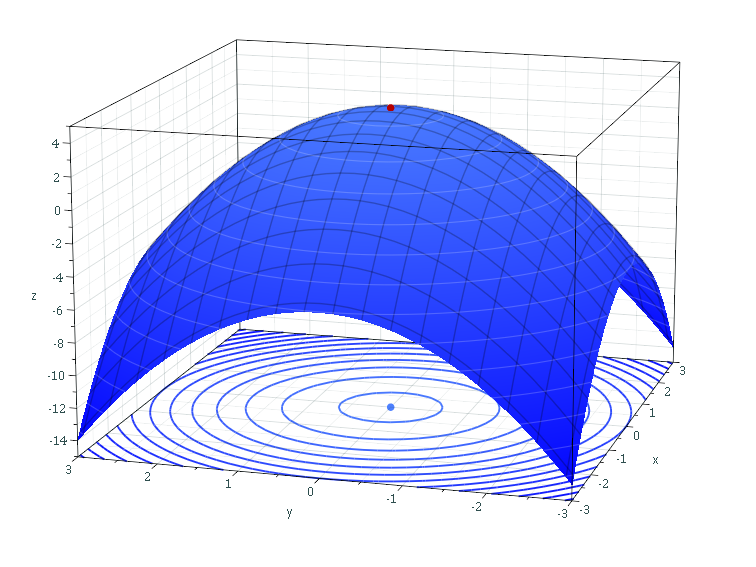
\includegraphics[width=0.6\textwidth]{images/MaximumParaboloid}
      \caption{Quelle: Wikipedia: https://en.wikipedia.org/wiki/File:MaximumParaboloid.png}
    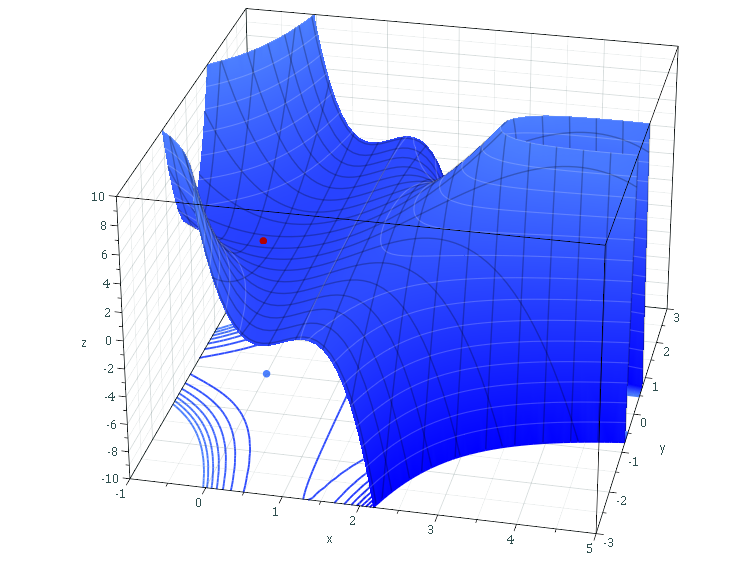
\includegraphics[width=0.6\textwidth]{images/MaximumCounterexample}
      \caption{Quelle: Wikipedia: https://en.wikipedia.org/wiki/File:MaximumCounterexample.png}
\end{figure}


\begin{Satz}[Notwendiges Kriterium]
 Ist $f: U  \to \mathbb{R}$ differenzierbar und hat  $f$ in $a \in U$ ein lokales Extremum, so gilt 
\begin{align*}
\frac{\partial}{\partial x_{1}}f(a)  = \cdots  = \frac{\partial}{\partial x_{n}} f(a) = 0 \;.
\end{align*}
Dies ist gleichbedeutend mit $df(a) = 0$.
\end{Satz}
\begin{proof}
Setze $F_k(t) := f(a + t e_k)$. Da $f$ ein Extremum in $a$ hat, hat $F_k$ in einer hinreichend kleinen Umgebung um $0$ ein Extremum. 
Da $F_k$ eine Funktion einer Veränderlichen ist, gilt $F'(0) = 0$. Da $\frac{\partial}{\partial x_k} f(a) = F_k'(0)$ folgt die Behauptung.
\end{proof}

\begin{Definition}[Kritischer Punkt]
Ein Punkt $a$ mit $df(a) = 0$ wird als kritischer Punkt Bezeichnet. 
\end{Definition}

\begin{Satz}[Hinreichendes Kriterium]
 Ist $f: U  \to \mathbb{R}$ eine $\mathcal{C}^2$-Funktion und ist $f'(a) = 0$  ein kritischer Punkt für ein $a \in U$. Dann gilt:
\begin{itemize}
\item $f''(a) > 0 \Rightarrow $ $f$ hat in $a$ ein isoliertes lokales Minimum.
\item $f''(a) < 0 \Rightarrow $ $f$ hat in $a$ ein isoliertes lokales Maximum.
\item $f''(a) \gtrless 0 \Rightarrow $ $f$ hat in $a$ einen Sattelpunkt.
\end{itemize} 
\end{Satz}
\begin{proof}
Sei $f'(a) = 0$ und $f''(a) > 0$. Mit der Taylorformel gilt für hinreichend kurze Vektoren $h \in \mathbb{R}^n$
\begin{align*}
f(a + h) = f(a) + \frac{1}{2} h^T f''(a) h + R(h)
\end{align*}
mit $\lim_{h \to 0} \frac{R(h)}{ ||h||^2} = 0$. Für $||h|| \leq 1$ hat $ h^T f''(a) h $ sein Maximum $m$ auf dem Einheitskreis $\{ h \in \mathbb{R}^n \; | \; ||h|| = 1 \}$ da $f''(a) > 0$.
\begin{align*}
 h^T f''(a) h  = ||h|| \frac{1}{||h||} h^t  f''(a)  ||h|| \frac{1}{||h||} h \geq m ||h||^2 \;.
\end{align*}
Wir wählen $\epsilon$ so klein, dass $R(h) \leq \frac{m}{2}  ||h||^2$ gilt für $||h|| < \epsilon$  (was geht wegen Taylorformel).
Damit erhalten wir
\begin{align*}
f(a + h) \geq f(a) +  m ||h||^2 \;.
\end{align*}
und damit hat $f$ ein lokales Minimum in $a$.

Der Fall $f''(a) < 0$ wird mit Betrachtung von $-f$ durch den vorigen Fall bewiesen.

Es sei nun $f''(a) \gtrless 0$ und $v$ mit $v^T f''(a) v > 0$ und $w$ mit $w^T f''(a) w > 0$. Betrachten wir die Funktionen
\begin{align*}
F_v (t) := f(a + tv) \\
F_w(t) := f(a +tw)
\end{align*}
dann ist 
\begin{align*}
F_v' (t) = 0; \; F_v''(0) = v^T f''(a) v > 0 \\
F_w' (t) = 0; \; F_w''(0) = w^T f''(a) w < 0 \\
\end{align*}
und somit hat $F_v$ ein isoliertes lokales Maximum und $F_w$ ein isoliertes lokales Minimum und damit $f$ kein lokales Extremum  in  $a$.
\end{proof}


\begin{figure}[H]
      \centering
    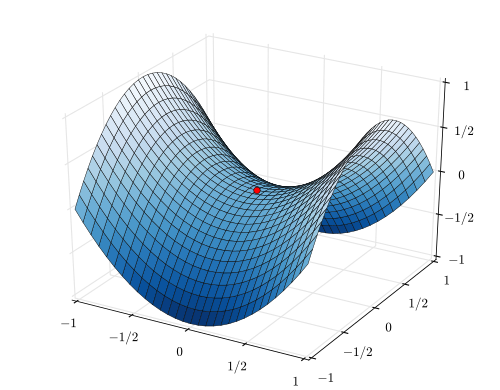
\includegraphics[width=0.6\textwidth]{images/Saddle_point}
      \caption{Quelle: Wikipedia: https://commons.wikimedia.org/wiki/File:Saddle\_point.svg}

\end{figure}



\subsubsection*{Anwendung: Gradientenverfahren} 
Wie kann man Minima einer  differenzierteren Abbildung $f: \mathbb{R}^n \to \mathbb{R}$ finden? 
Wir wissen, dass an jedem Punkt $x_k \in : \mathbb{R}^n$ der negative Gradient  $d_k := -\nabla f (x_k)$ in die steilste Abstiegsrichtung zeigt.
Die Idee des Gradientenabstieg ist, ein bestimmtes  Stück in diese Richtung abzusteigen, damit der Funktionswert kleiner wird, also $x_{k+1} = x_k + \alpha_k d_k$ zu setzen. Für hinreichend kleines $\alpha_k$ folgt mit Satz \ref{lokaleLinearisierung} über die lokale Liberalisierung  
$f(x_{k+1}) = f (x_k + \alpha_k d_k) =  f(x_k) + \alpha_k df(x_k)d_k + R( \alpha_k dk)$.  Somit gilt $f(x_{k+1}) \leq f(x_k)$, falls $\nabla f(x_k) \neq 0$ und falls die folge $f(x_k)$ beschränkt ist, so ist  dieser Fixpunkt $x^*$ ein minimum, da $\nabla f(x^*) = 0$ gelten muss.  

\begin{algorithm}
\caption{Gradientabstieg}
\begin{algorithmic}[1]


    \State Initialisiere $k:=0$ und zufälligen Startwert $x_0$.
\State Initialisiere Genauigkeit $\epsilon > 0$.
    \While{$|| \nabla f(x_k) || > \epsilon$}  \Comment{So lange kein Extrema vorliegt}
        \State Bestimme $\alpha_k$  mit $f (x_k + \alpha d_k) =  f(x_k) + \alpha_k df(x_k)d_k + R( \alpha_k dk)$ \Comment{Schrittweite bestimmen}
        \State Setze $x_{k+1} := x_k  + \alpha_k d_k$. \Comment{Absteigen}
 	\State  $k \leftarrow k+1$ \Comment{Wiederholen}
    \EndWhile  \label{Gradientenverfahren}


\end{algorithmic}
\end{algorithm}

\begin{figure}[H]
      \centering
    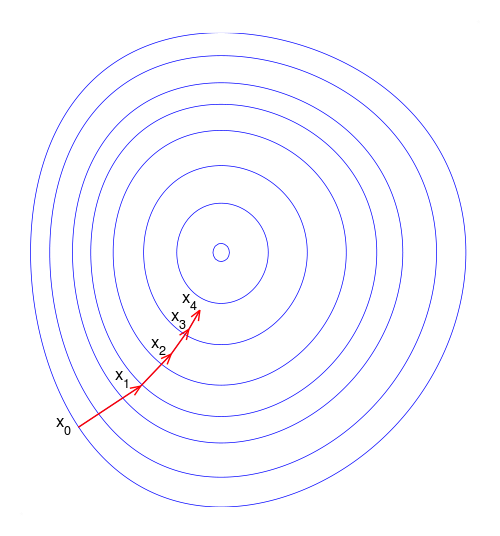
\includegraphics[width=0.7\textwidth]{images/Gradient_descent}
      \caption{Quelle: Wikipedia}
\end{figure}



\begin{Definition}
Sei  $f: \mathbb{R}^n \to \mathbb{R}$  eine differenzierbare Funktion. Eine Kurve $\gamma : I \to \mathbb{R}^n$, auf der $f$ konstant ist, also 
$f(\gamma(t)) = c$ für eine festes $c \in \mathbb{R}$ gilt, heißt Höhenlinie.
\end{Definition}

\begin{Bemerkung}
Der Gradient steht senkrecht auf  Höhenlinien. Dies bedeutet, dass $$ \bigl \langle \nabla f(\gamma(t)), \gamma'(t) \bigr \rangle = 0$$ gilt. 
\end{Bemerkung}
\begin{proof}
Aus $f(\gamma(t)) = c$ folgt $\frac{d}{dt} f(\gamma(t)) = 0$. Mit der Kettenregel folgt $\frac{d}{dt} f(\gamma(t)) =  f(\gamma(t)) \cdot \gamma'(t) = 0$ und damit
$ \bigl \langle \nabla f(\gamma(t)), \gamma'(t) \bigr \rangle = 0$.
\end{proof}

\subsubsection*{Anwendung: Backpropagation}
Ein Neuronales Netz ist eine Funktion $f : \Omega \times \mathbb{R}^n \to \mathbb{R}^m$, die einem Input (auch Feature genannt) in Abhängigkeit der Gewichte $\Omega$
einen Ausgabewert zuordnet. Die Funktion ist dabei aus einfachen Bausteinen zusammengesetzt.

\begin{figure}[H]
      \centering
    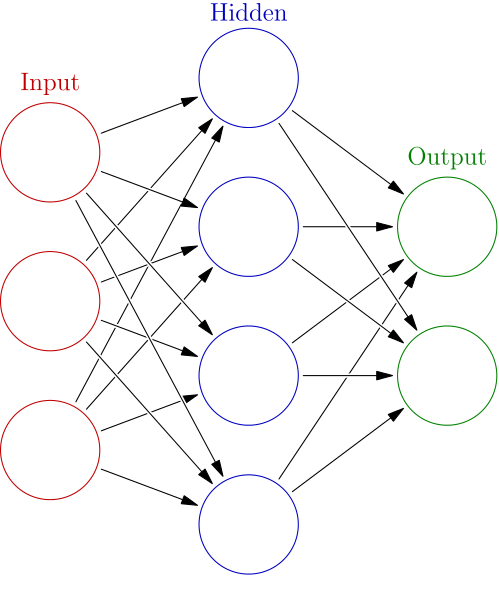
\includegraphics[width=0.4\textwidth]{images/499px-Colored_neural_network}
      \caption{Quelle: Wikipedia}
    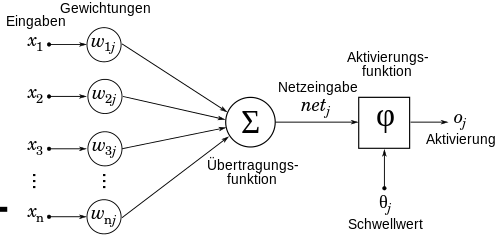
\includegraphics[width=0.6\textwidth]{images/500px-NeuronModel_deutsch}
      \caption{Quelle: Wikipedia}
\end{figure}


Gegeben ist ein  Datensatz $D : = \{ (x_i, y_i) \}$. Finde Gewichte Omega, so dass Lossfunktion
\begin{align*}
L_D  : \Omega \subset \mathbb{R}^n \to \mathbb{R} 
\end{align*}
minimal wird. Zum Beispiel $L_D(\omega) := \sum_{(x_i,y_i) \in D} (f(\omega, x_i) - y_i)^2$.

Wende Gradientenverfamren an:

\begin{algorithm}
\caption{Gradientabstieg}
\begin{algorithmic}[1]
    \State Initialisiere $k:=0$ und zufällige Gewichte $w_0$.
\State Initialisiere Genauigkeit $\epsilon > 0$.
    \While{$|| \nabla L_D(\omega) || > \epsilon$}  \Comment{So lange kein Extrema vorliegt}
        \State Bestimme $\alpha_k$  mit $ L_D(\omega_k + \alpha d_k) =  L_D(\omega_k) + \alpha_k d L_D(\omega_k)d_k + R( \alpha_k dk)$ \Comment{Schrittweite bestimmen}
        \State Setze $\omega_{k+1} := \omega_k  + \alpha_k d_k$. \Comment{Absteigen}
 	\State  $k \leftarrow k+1$ \Comment{Wiederholen}
    \EndWhile  \label{roy's loop}


\end{algorithmic}
\end{algorithm}

Wenn der Datensatz $D$ sehr groß ist (Big Data), ist die Berechnung des Gradient der Lossfunktion entsprechend aufwendig. Um diesen Aufwand zu reduzieren,
kann man das Gradientenverfamren modifizieren, so dass man Gradienten nur auf Teilräumen berechnet. Man erhält somit das sogenannte Mini-Batch Gradientenverfamren und das stochastische Gradientenverfamren.

\begin{algorithm}
\caption{Gradientabstieg}
\begin{algorithmic}[1]
    \State Initialisiere $k:=0$ und zufällige Gewichte $w_0$.
\State Initialisiere Genauigkeit $\epsilon > 0$.
\State Wähle Teilmenge $D_0' \subset D$
    \While{$|| \nabla L_{D'_0}(\omega) || > \epsilon$}  \Comment{So lange kein Extrema vorliegt}
        \State Bestimme $\alpha_k$  mit $ L_{D'_0}(\omega_k + \alpha d_k) =  L_{D'_0}(\omega_k) + \alpha_k d L_{D'_0}(\omega_k)d_k + R( \alpha_k dk)$ \Comment{Schrittweite bestimmen}
        \State Setze $\omega_{k+1} := \omega_k  + \alpha_k d_k$. \Comment{Absteigen}
	\State Wähle neue Teilmenge $D'_{k +} \subset D$.
 	\State  $k \leftarrow k+1$ \Comment{Wiederholen}
    \EndWhile  \label{roy's loop}


\end{algorithmic}
\end{algorithm}

Wenn man als Teilmenge immer nur eine einelementige Menge wählt, so spricht man vom stochastischen Gradientenverfahren.

\begin{figure}[H]
      \centering
    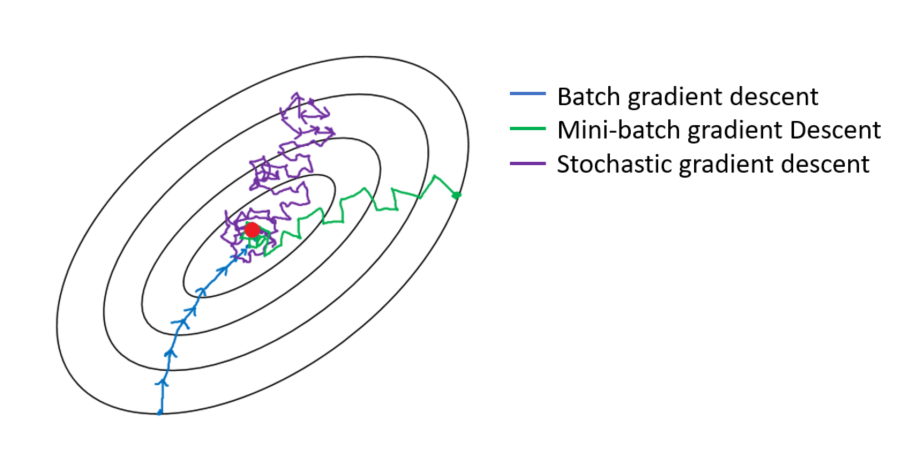
\includegraphics[width=1.0\textwidth]{images/batchgradient}
      \caption{Quelle: https://towardsdatascience.com/batch-mini-batch-stochastic-gradient-descent-7a62ecba642a}

\end{figure}


\subsection{Gradient einer  mehrdimensionalen Funktion}
\begin{Definition}
\label{diffbarkeitmd}
Eine Funktion $F: U \to \mathbb{R}^m$ heißt differenzierbar, wenn es eine lineare Abbildung $dF$ gibt, so dass 
\begin{align*}
F(a + h) = F(a) + dF(a)h + R(h)
\end{align*}
mit $\lim_{h \to 0} \frac{R(h)}{||h||} = 0$ gilt für alle $a \in U$ und $h \in \mathbb{R}^n$.
\end{Definition}

\begin{Bemerkung}
Im Fall $n = 1$ stimmt diese Definition mit der Alten Definition \ref{diffbarkeit} überein.
\end{Bemerkung}
\begin{proof}
Nach Satz \label{lokaleLinearisierung} gilt für eine differenzierbare Funktion $f(a + th) = f(a) + df th + R(th)$ mit  $\lim{t \to 0} \frac{R(th)}{||h||} = 0$. Umstellen ergibt
\begin{align*}
df(a) h = \lim_{t \to 0} \frac{f(a + th) - f(a)}{t}
\end{align*} 
und somit existieren alle linearen Abbildungen und wegen der Linearität von $df$ sind diese auch stetig.
\end{proof}

\begin{Beispiel}[Affine Abbildung]
Für $A \in \mathbb{R}^{n \times n}$, $b \in \mathbb{R}^n$  ist die Abbildung $F(x) := Ax +b$ differenzierbar, da
$F(a +h) = A(a+h) + b = A a+ Ah +b = Aa +b + Ah = F(a) + Ah$ und damit für $dF(a) := A$ und $R(h) = 0$ die Definition \ref{diffbarkeitmd}
 erfüllt ist.
\end{Beispiel}

\begin{Satz}[Differenzierbarkeit von Produktfunktionen]
Eine Funktion $F:= (F_1, F_2) : U  \to \mathbb{R}^m \times \mathbb{R}^k$ ist genau dann differenzierbar, 
wenn $F_1 : U  \to \mathbb{R}^m$ und   $F_2 : U  \to \mathbb{R}^k$ differenzierbar sind. In diesem Fall ist
$$dF(a) = (dF_1(a), df_2 (a)) \;.$$ 
\end{Satz}
\begin{proof}
Sind $F_1$ und $F_2$ differenzierbar, so gilt für $i = 1,2$
\begin{align*}
F_i (a + h) = F_i(a) + dF_ih + R_i(h)
\end{align*}
Dann gilt mit $dF(a) = (dF_1(a), df_2 (a))$ und $R(h):= (R_1(h), R_2(h))$
\begin{align*}
F (a + h) = F (a) + dF h + R(h)
\end{align*}
mit $\lim_{h \to 0} \frac{R(h):}{||h||} = 0$ und damit ist $F$ differenzierbar. Die Umkehrung folgt analog.
\end{proof}

\begin{Bemerkung}[Differenzial von  Produkfunktionen]
Eine Abbildung $F : U \to \mathbb{R}^m$ ist genau dann  differenzierbar, wenn ihre Koordinaten-Funktionen 
$F_1 : U \to \mathbb{R},  \cdots, F_m : U \to \mathbb{R}$ mit $F(a) = \begin{pmatrix} F_1(a) \\ \vdots \\ F_m(a) \end{pmatrix}$ differenzierbar sind. In diesem Fall gilt
\begin{align*}
dF(a) :=   \begin{pmatrix}  \frac{\partial}{\partial x_1}  F_1(a) & \cdots & \frac{\partial}{\partial x_n} F_1(a) \\ 
\vdots & & \vdots \\
\frac{\partial}{\partial x_1}  F_m(a) & \cdots & \frac{\partial}{\partial x_n} F_m(a) 
\end{pmatrix}
\end{align*}
\end{Bemerkung}

\begin{Bemerkung}[Differenzierbarkeit von Wegen]
Ein Weg $\gamma =  \begin{pmatrix} \gamma_1  \\ \vdots \\ \gamma_m \end{pmatrix} : I \to U$ ist genau dann differenzierbar, wenn $\gamma_i$ differenzierbar ist für $i= 1, \cdots, m$ und dann gilt $\gamma'(t) =   \begin{pmatrix} \gamma'_1(t)  \\ \vdots \\ \gamma'_m(t) \end{pmatrix} \; .$
\end{Bemerkung}



\begin{Satz}[Kettenregel]
Seien $G:  U \subset \mathbb{R}^n \to V \subset \mathbb{R}^m$ und $F: V \to Z \subset \mathbb{R}^k$ differenzierbar. Dann ist $F \circ G$ differenzierbar und mit $b := G(a)$ es gilt
$$ d(F \circ G)(a) = dF(b) \cdot dG(a) $$
\end{Satz}
\begin{proof}
Analog zu Baby Kettenregel.
\end{proof}


\subsubsection*{Anwendung: Automatisches Ableiten} 


\begin{figure}[H]
      \centering
    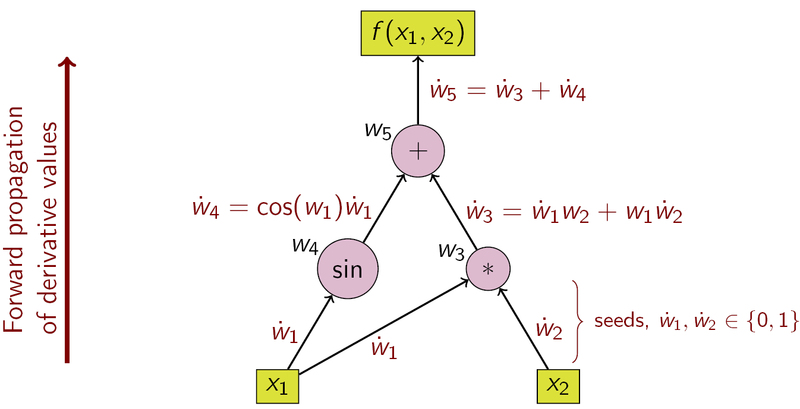
\includegraphics[width=0.8\textwidth]{images/ad.png}
      \caption{Quelle: Wikipedia}
\end{figure}

\href{https://pytorch.org/tutorials/beginner/blitz/autograd_tutorial.html}{Automatisches Ableiten  in Pytorch}


Mit Hilfe des Automatischen Ableiten kann man den Gradienten der Lossfunktion zu einem Neuroyalen Netzt einfach berechnen, da dieser sich aus einfachen Funktionen zusammensetzt.








\section{Mehrdimensionale Integralrechnung}

\subsection{Lebesgue Maß}
Für Intervalle $I_i : = (a_i,b_i) \subset \mathbb{R}$ nennen wir $I := I_1 \times \cdots \times I_n$ einen Quader und definieren sein Volumen
\begin{align*}
\text{vol}_n (I):=   \prod_{i = 1}^n (b_i -a_i)  
\end{align*}
Mit $I(n): = \{   I_1 \times \cdots \times I_n  \; | \;  I_i := (a_i, b_i) \subset \mathbb{R} \}$ bezeichnen wir die Menge aller $n$-dimensionalen Quader. 
\begin{Definition}
Für eine Menge $A \subset \mathbb{R}^n$ definieren wir das Lebuesgsche äußere Maß
\end{Definition}
\subsection{Lebesgue Integral}

\subsubsection*{Anwendung: Fourierreihen, Fouriertransformation und FFT} 

%back
\newpage
\listoftables{\addcontentsline{toc}{section}{\listtablename}}
\newpage
\listoffigures{\addcontentsline{toc}{section}{\listfigurename}}
\newpage
\IfDefined{printindex}{\printindex}
\IfDefined{printnomenclature}{\printnomenclature[4.5cm]{}}
\end{document}
